\section{Linguistic Motivation and BSML Semantics}\label{Motivation}

BSML (Bilateral State-Based Modal Logic) originates from a project led by Aloni, 
titled N$\varnothing$thing is Logical (NihiL)\footnote{For details, see \url{https://www.marialoni.org/Nihil}.}. 
This project concerns formal semantics. It is a field that uses formalized methods to analyze semantic phenomena and seeks to uncover the underlying rules about how meanings of complex expressions are built from their parts.
Natural language, as used in daily communication, often does not conform to classical logic. Consequently, formal semanticists develop non-classical logical systems to better capture linguistic phenomena.

BSML was initially designed to address a well-known issue in linguistics: free choice (FC). Consider the following sentence:

\begin{quote}
    You may go to the beach or to the cinema.
\end{quote}

In natural language, this typically allows the inference:

\begin{quote}
    You may go to the beach, and you may go to the cinema.
\end{quote}

However, in classical modal logic, this inference does not hold. Specifically, from $\Diamond (a \vee b)$, we cannot derive $\Diamond a \land \Diamond b$.

A common strategy in semantics is to attribute certain inferences to pragmatics. 
That is, while semantics concerns literal meaning, pragmatics examines how meaning is shaped by context. For instance, if one says:

\begin{quote}
    Some students in this class are studying logic.
\end{quote}

Listeners typically infer that not all students are studying logic——otherwise, the speaker would have simply stated, ``All students are studying logic''.
This inference is not a semantic entailment but rather a pragmatic inference.


Similarly, in the case of free choice, 
Aloni's approach to free choice is based on the idea that speakers construct mental models of reality when interpreting sentences. 
Her central claim (see \citet{Aloni2022}), termed \textbf{Neglect-Zero}, is as follows
\begin{quote}
    \textbf{Neglect-Zero:} 
     When interpreting a sentence, speakers construct mental models of reality.In doing so, they systematically neglect structures that satisfy the sentence through an empty configuration (zero-models).
    
\end{quote}
Intuitively, this means that when interpreting a disjunction, speakers ignore the possibility of an empty disjunct.\@

Here, we introduce several key non-classical semantics in BSML.\@ The full definitions will be provided in the next chapter.\@


First, BSML formalizes this tendency by introducing the \textit{nonemptiness atom} (NE), which ensures that only nonempty states are considered in the interpretation of sentences. 
The NE operator is defined as follows:  

\begin{quote}
    \textbf{Nonemptiness Atom (NE):} 
    \begin{itemize}
        \item \textbf{Support Condition:} $M, s \models \text{NE}$ iff $s \neq \varnothing$.
        \item \textbf{Anti-Support Condition:} $M, s \leftmodels \text{NE}$ iff $s = \varnothing$.
    \end{itemize}
\end{quote}


    The operator NE is used to define a pragmatic enrichment function \({[ \quad]}^+\), which is not inherently part of the logical system, 
    but the introduction of NE enables us to formally capture and implement this pragmatic effect within the logic system.:


\begin{align*}
    {[p]}^+ &= p \land \text{NE} \\
    {[\neg \alpha]}^+ &= \neg {[\alpha]}^+ \land \text{NE} \\
    {[\alpha \lor \beta]}^+ &= ({[\alpha]}^+ \lor {[\beta]}^+) \land \text{NE} \\
    {[\alpha \land \beta]}^+ &= ({[\alpha]}^+ \land {[\beta]}^+) \land \text{NE} \\
    {[\Diamond \alpha]}^+ &= \Diamond {[\alpha]}^+ \land \text{NE}
\end{align*}

Second, BSML is built upon team semantics, meaning that formulas are evaluated with respect to sets of possible worlds (teams) rather than individual worlds. 
For example, in Figure\ref{disjunct}, the black small square represents a state in a universe.
And (b) is the zero-model of \( a \vee b \), because one of the disjunctors is empty.

\begin{figure}[h]
    \centering
    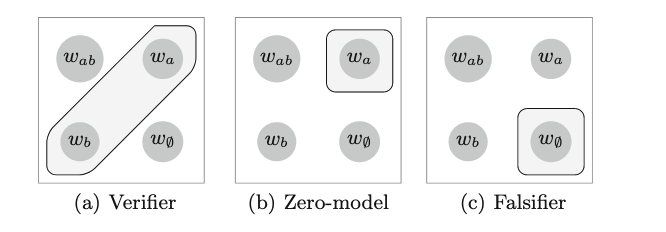
\includegraphics[width=\textwidth]{image/disj1.png}
    \caption{Models for \( a \vee b \)}\label{disjunct}
\end{figure}

Additionallt, BSML relies on a bilateral semantics, where each formula has both \textbf{support/assertion conditions ($\models$)} and \textbf{anti-support/rejection conditions ($\leftmodels$)}.

\begin{quote}
    $M, s \models \varphi$: \( \varphi \) is assertable in information state \( s \), with \( s \subseteq W \).

    $M, s \leftmodels \varphi$: $\varphi$ is rejectable in information state $s$, with $s \subseteq W$.
\end{quote}

And logical consequence is defined as preservation of support. 

\begin{quote}
\(\varphi \models \psi\) \quad \text{iff} \quad $\forall M, s : M, s \models \varphi \Rightarrow M, s \models \psi$
\end{quote}

Based on team-semantics, BSML adopts a split disjunction based on state-based semantics:

\begin{quote}
    $M, s \models \varphi \vee \psi \colon \Leftrightarrow$ there exist $t, u$ such that $s = t \cup u$ and $M, t \models \varphi$ and $M, u \models \psi$.
    
    $M, s \leftmodels \varphi \vee \psi \colon \Leftrightarrow M, s \leftmodels \varphi$ and $M, s \leftmodels \psi$.
\end{quote}


BSML can be extended with global disjunction:
\begin{itemize}
    \item \(\textbf{BSML}^{\inqdisj}\): This extension adds the \textit{global disjunction} \(\inqdisj\), which allows for the expression of properties that are invariant under bounded bisimulation.
\end{itemize}

The global disjunction also called inquisitive disjunction. 
Inquisitive semantics commonly employs a global disjunction to capture questions. 


With these approach, we establish a robust logical framework capable of predicting linguistic phenomena. 
By comparing these predictions with actual language usage in the real world, we can gain valuable insights into the underlying mechanisms of language.


It is easy to see that pragmatic enrichment has a non-trivial effect on disjunctions, 
and it has non-trivial effects only on disjunctions and only if they occur in a positive environment. 
In other words, the effect of Neglect-Zero is restricted to disjunction sentences, vanishing under negation but reappearing under double negation.
The following are some linguistic properties, which are crucial for understanding the system's behavior and its implications for free choice inferences:

\begin{itemize}
    \item \textbf{Narrow Scope FC:} \quad ${[ \Diamond (\alpha \lor \beta) ]}^+ \models \Diamond \alpha \land \Diamond \beta$
    \item \textbf{Wide Scope FC:} \quad ${[\Diamond \alpha \lor \Diamond \beta]}^+ \models \Diamond \alpha \land \Diamond \beta$ 
          \quad (if $R$ is indisputable)
    \item \textbf{Dual Prohibition:} \quad ${[\neg \Diamond (\alpha \lor \beta)]}^+ \models \neg \Diamond \alpha \land \neg \Diamond \beta$
    \item \textbf{Double Negation:} \quad ${[\neg \neg \Diamond (\alpha \lor \beta)]}^+ \models \Diamond \alpha \land \Diamond \beta$
 \end{itemize}
 
 This project adopts \(\textbf{BSML}^{\inqdisj}\), and the following is the specific Haskell implementation.
   